\documentclass[11pt,a4paper]{article}
\usepackage[margin=1in]{geometry}
\usepackage{amsmath,amssymb}
\usepackage{graphicx}
\usepackage{booktabs}
\usepackage{hyperref}
\usepackage{enumitem}
\usepackage{xcolor}
\usepackage{float}

\graphicspath{{plots/}}
\hypersetup{colorlinks=true, linkcolor=blue, urlcolor=blue, citecolor=blue}

\title{EE675 Assignment 2: Policy Gradient for Predator-Prey Game}
\author{Shreyash}
\date{}

\begin{document}
\maketitle

\section{Problem setting and simulator convention}
This assignment uses the same predator-prey environment as Assignment 1, with grid size fixed at $N=4$ and discount factor $\gamma=0.99$. A state is written as
\[
    S_t = \big((x_t^p,y_t^p),(x_t^q,y_t^q)\big),
\]
where $(x_t^p,y_t^p)$ is the predator position and $(x_t^q,y_t^q)$ is the prey position. The predator starts at $(1,1)$ and the prey starts at $(N,N)$. The five global actions are
\[
    \mathcal{A}=\{\texttt{stay},\texttt{up},\texttt{down},\texttt{left},\texttt{right}\}.
\]

The one-step simulator follows the same convention used in my Assignment 1 code. The predator moves first. If it reaches the prey, the reward is $1$ and the prey respawns uniformly over the remaining $N^2-1$ cells. If the predator does not catch the prey immediately, the prey moves uniformly over its feasible one-step positions, including staying in place, and the catch condition is checked again. If no catch occurs, the reward is $0$.

For invalid boundary moves, the simulator itself uses the Assignment 1 convention that the agent remains in the same cell. During policy-gradient training, however, I mask invalid predator actions before sampling from the neural policy. Thus, the network still outputs logits for all five global actions, but the sampled action is drawn only from the feasible actions at the current predator location. This avoids assigning probability mass to boundary moves that would not change the predator's position.

\section{Neural policy design}
The policy $\pi_\theta(a\mid s)$ is implemented in \texttt{policy\_network.py} using PyTorch. I encode each state by normalized coordinates:
\[
    \phi(s)=\left[\frac{x^p-1}{N-1},\frac{y^p-1}{N-1},\frac{x^q-1}{N-1},\frac{y^q-1}{N-1}\right] \in \mathbb{R}^4.
\]
The input dimension is therefore $4$. The output dimension is $5$, one logit for each action in $\mathcal{A}$. I used the architecture
\[
    4 \rightarrow 64 \rightarrow 64 \rightarrow 5,
\]
with \texttt{Tanh} nonlinearities after the two hidden layers. I kept the network small because the state representation is only four-dimensional and the grid is fixed at $4\times4$ for this assignment.

Given a state, the network produces unnormalized logits. Invalid predator actions are assigned a very negative logit before constructing a categorical distribution. The final action distribution is therefore
\[
    \sum_{a\in\mathcal{A}(s)} \pi_\theta(a\mid s)=1,
\]
where $\mathcal{A}(s)$ denotes the feasible predator actions at state $s$.

\section{Policy-gradient estimator}
Although the game is continuing, the implementation uses a finite rollout horizon $H$. The truncated discounted objective is
\[
    J_H(\theta)=\mathbb{E}_{\tau\sim\pi_\theta}\left[\sum_{t=0}^{H-1}\gamma^t R_{t+1}\right].
\]
In the code, the reward returned after taking action $A_t$ is stored as \texttt{rewards[t]}; in standard notation this corresponds to $R_{t+1}$.

For a sampled trajectory, define the return-to-go
\[
    G_t = \sum_{k=t}^{H-1}\gamma^{k-t}R_{k+1}.
\]
Using the likelihood-ratio identity, the finite-horizon policy gradient can be written as
\[
    \nabla_\theta J_H(\theta)
    = \mathbb{E}\left[\sum_{t=0}^{H-1}\gamma^t G_t\,\nabla_\theta\log\pi_\theta(A_t\mid S_t)\right].
\]
With $M$ independently sampled trajectories, I use the Monte Carlo estimate
\[
    \widehat{g}
    = \frac{1}{M}\sum_{i=1}^{M}\sum_{t=0}^{H-1}\gamma^t G_t^{(i)}
    \nabla_\theta\log\pi_\theta(A_t^{(i)}\mid S_t^{(i)}).
\]
This is an unbiased estimator of the policy gradient for the truncated objective $J_H(\theta)$, assuming the trajectories are sampled from the current policy.

The score-function term is computed using
\[
    \texttt{torch.distributions.Categorical.log\_prob(action)}.
\]
The gradients of the REINFORCE surrogate objective are then obtained using
\[
    \texttt{torch.autograd.grad(objective, policy.parameters())}.
\]
This implementation is in \texttt{gradient\_estimate.py}.

\section{Simple stochastic gradient ascent}
The manual stochastic gradient ascent update is
\[
    \theta_{k+1}=\theta_k+\eta\widehat{g}_k.
\]
This is implemented in \texttt{simple\_sga.py} by directly adding the estimated gradient to each parameter tensor under \texttt{torch.no\_grad()}. For the reported run, I used
\[
    \eta_{\text{SGA}}=0.02.
\]
The run used $100$ iterations, $M=4$ trajectories per update, rollout horizon $H=60$, and $\gamma=0.99$. I kept $M$ small to keep the runtime manageable, so the learning curve is expected to be noisy.

\begin{figure}[H]
    \centering
    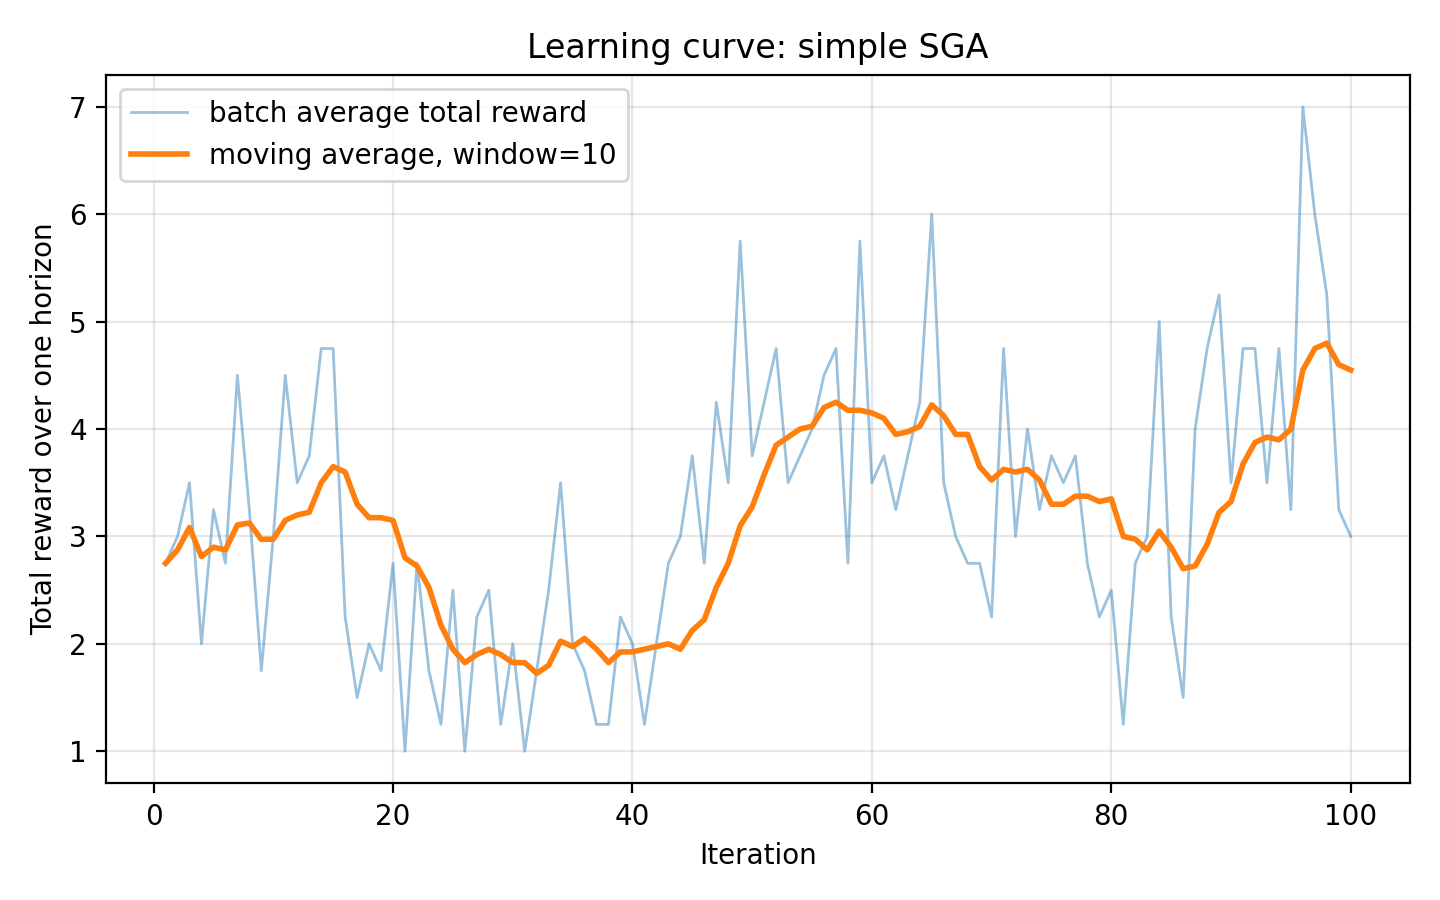
\includegraphics[width=0.82\textwidth]{simple_sga_learning_curve.png}
    \caption{Learning curve for simple stochastic gradient ascent. Each point is the average total reward over the sampled trajectories in that update; the smoothed curve is more informative than any single noisy iteration.}
\end{figure}

\section{Adam optimizer}
I also trained the same neural policy using PyTorch's \texttt{torch.optim.Adam}. Since PyTorch optimizers minimize by default, I minimized the negative REINFORCE surrogate objective. Thus, the Adam code performs gradient ascent on the same policy-gradient objective as simple SGA.

For Adam, I used
\[
    \eta_{\text{Adam}}=0.001.
\]
The other settings were unchanged: $100$ iterations, $M=4$, $H=60$, and $\gamma=0.99$.

\begin{figure}[H]
    \centering
    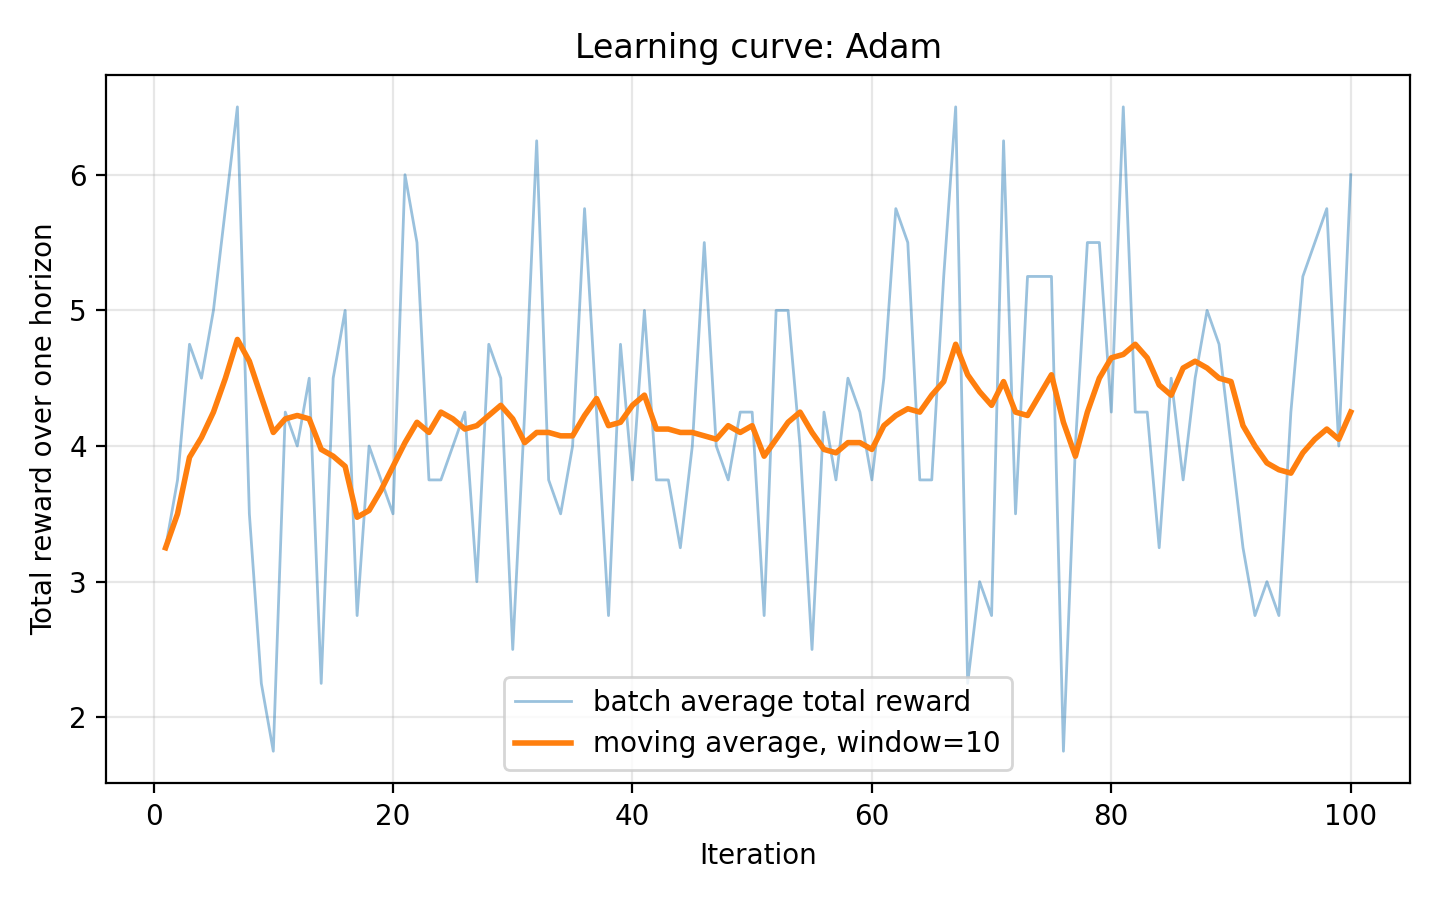
\includegraphics[width=0.82\textwidth]{adam_learning_curve.png}
    \caption{Learning curve for Adam. The curve is still stochastic because the updates are based on simulator rollouts, but Adam handles the gradient scale automatically through its adaptive moment estimates.}
\end{figure}

\section{Numerical observations}
The table below reports diagnostics from \texttt{results/training\_log.csv}. The plotted reward is the average undiscounted total reward collected over one rollout horizon, averaged over the trajectories sampled for that update.

\begin{table}[H]
\centering
\begin{tabular}{lrrrrr}
\toprule
Method & First reward & Last reward & Last-10 avg. & Max reward & Last-10 discounted avg. \\
\midrule
simple SGA & 2.75 & 3.00 & 4.55 & 7.00 & 3.448 \\
Adam & 3.25 & 6.00 & 4.25 & 6.50 & 3.131 \\
\bottomrule
\end{tabular}
\caption{Summary of the generated learning curves. Because rewards are sparse and only a small Monte Carlo batch is used, the reward is not monotone across iterations.}
\end{table}

Both optimizers improve over the initial behavior, but the trajectories remain noisy. In this run, Adam ends with a higher final batch reward, while simple SGA attains a slightly higher maximum reward and a slightly higher last-10 average. Since each point is computed from fresh simulator rollouts, I interpret these plots mainly as evidence that policy-gradient training is working, not as a precise optimizer ranking.

\section{Code organization and reproduction}
The code is split by functionality:
\begin{itemize}[noitemsep]
    \item \texttt{environment.py}: simulator, action utilities, valid-action logic, and prey respawn.
    \item \texttt{policy\_network.py}: state encoder, neural policy, and masked categorical action distribution.
    \item \texttt{gradient\_estimate.py}: rollout sampling and REINFORCE gradient estimation.
    \item \texttt{simple\_sga.py}: manual stochastic gradient ascent update.
    \item \texttt{train.py}: training loops for simple SGA and Adam, CSV logging, and plot generation.
\end{itemize}

To reproduce the reported run, install the dependencies and execute
\begin{verbatim}
pip install -r requirements.txt
python train.py --iterations 100 --episodes 4 --horizon 60 \
                --sga-lr 0.02 --adam-lr 0.001
\end{verbatim}
This regenerates \texttt{results/training\_log.csv}, \texttt{plots/simple\_sga\_learning\_curve.png}, and \texttt{plots/adam\_learning\_curve.png}.

\end{document}
